\chapter{Conceitos Básicos}

%source: http://epos.lisha.ufsc.br/EPOS+User+Guide
\section{EPOS}

EPOS (Embedded Parallel Operating System) é um sistema operacional orientado a aplicação, cujo design chama-se ADESD (\emph{Application-Driven Embedded System Design Method}), proposto por Fröhlich \cite{guto_thesis}. A ideia central do EPOS é prover um sistema operacional mínimo, de modo a minimizar o \emph{overhead} da existência de um sistema operacional, deixando o processador livre para executar a aplicação do desenvolvedor \cite{epos_user_guide}.

Como o objetivo é criar um ambiente em que o desenvolvedor possa rapidamente produzir suas aplicações, EPOS provê vários utilitários comumente usados em aplicações, como filas, listas, tabelas de hashs, vetores, semáforos, OStream (para imprimir na tela), números aleatórios, cálculo de CRC e etc. Além destes utilitários, EPOS também provê uma série de componentes como threads, alarmes, cronometros, \emph{heaps} e meios para acessar a rede (internet).

\section{Arquitetura do EPOS}

\textbf{Mediadores de Hardware:} Dentro da arquitetura do EPOS há o conceito de mediadores de hardware, que são os componentes (ou classes) dependentes de plataforma. Idealmente, as únicas classes que precisam ser modificadas e/ou reimplementadas são os mediadores. Há mediadores específicos da placa, como por exemplo Pandaboard, Zedboard e etc; abstraídos sob o nome de \emph{machine} e mediadores específicos de um processador, abstraídos sob o nome de \emph{architecture}. No código do EPOS, estes mediadores encontram-se nas pastas \emph{mach} e \emph{arch}.
% Fonte: Hardware Mediators: A Portability Artifact for Component-based Systems
% HAL vs Virtualização vs Mediadores

Mediadores de hardware são uma alternativa ao tradicional uso de VMs\footnote{Virtual Machines.} e de HAL\footnote{Hardware Abstraction Layer}, proposta por Fröhlich em seu trabalho \emph{Application-Oriented System Design} \cite{guto_thesis}. O problema do uso de VMs é o seu \emph{overhead} causado devido à tradução das operações da VM em código nativo. Já o uso de um HAL incorre no problema da manutenibilidade e dificuldade de adapção à novas arquiteturas muito distintas entre si \cite{hw_mediators}. O HAL não conseguiu passar pela ``prova do tempo'', e já está sendo considerado obsoleto por distribuições GNU/Linux populares, como o 
Ubuntu\footnote{\url{http://www.linux-magazine.com/Online/News/Ubuntu-10.04-Alpha-2-Removes-HAL}}, sendo chamado de ``uma grande não-manutenível bagunça monolítica''\footnote{\url{https://wiki.ubuntu.com/Halsectomy}}.



\textbf{Traits:} Traits são classes onde é possível configurar certos componentes do EPOS em tempo de compilação. Lá é possível, por exemplo, definir o tamanho da \emph{stack} e \emph{heap} do sistema, a sua frequência de \emph{clock} bem como ativar ou desativar certas funções do sistema. Esta classe normalmente precisa ser alterada em um porte, mesmo ela não sendo um mediador de hardware, pois eles usam as configurações descritas nos traits.

\textbf{Interface Infladas: } Um conceito importante da arquitetura do EPOS é a Interface Inflada. %http://www.inf.ufsc.br/~guto/publications/aoos.pdf
Em sistemas orientados a aplicação, famílias de abstrações são frequentemente tratadas como entidades únicas, algo que pode ser vantajoso para o programador da aplicação, já que este não precisaria se preocupar com qual membro em específico desta família ele precisaria usar \cite{guto_thesis}.

Interface inflada basicamente é uma interface que declara os métodos de todas as classes que derivam dela, exportanto assim todos os métodos daquela família de abstrações, como mostra a figura \ref{fig:inflated}. Deste modo, o desenvolvedor de aplicativo poderia escrever a aplicação inteira em termos da interface inflada, relegando a tarefa de configuração do sistema a um utilitário automatizado. Tal utilitário poderia, através de uma análise sintática do código fonte, escolher quais os membros mais apropriados da família exportada serão associados no momento da compilação \cite[p.~56]{guto_thesis}.

%write about specifics from timers
\begin{figure}[ht!]
	\label{fig:inflated}
    \centering
    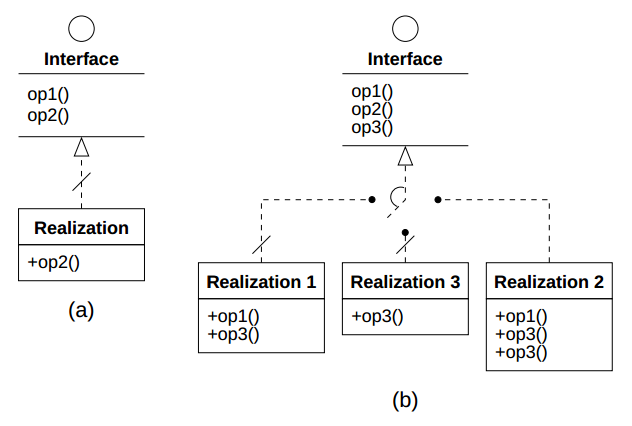
\includegraphics[width=7.5cm]{figuras/inflated_interface}
    \caption{Exemplos de uso de interfaces infladas \cite{guto_thesis}.}
\end{figure}


\section{Hardware-alvo}
%source: http://www.zedboard.org/product/zedboard
% http://www.zedboard.org/sites/default/files/documentations/ZedBoard_HW_UG_v2_2.pdf
Zedboard é uma plataforma de desenvolvimento que suporta uma grande variedade de aplicações, visto que ela possui uma boa gama de interfaces e funções para habilitar isto. É dedicada à prototipação e \emph{proof-of-concept}. Em seu interior ela possui um Xilinx Zynq 7000 (Z-7020), que é a arquitetura alvo deste porte. A figura \ref{fig:zed} mostra como é a placa fisicamente.

O ZYNQ-7000 SOC XC7Z020-CLG484-1 conta com o processador Dual ARM Cortex-A9 MPCore. O Zynq possui 4 graduações de velocidade de \emph{clock}, a comercial (graduação -1), industrial (graduação -1 a -2), estendida (-2 a -3) e expandida (-1), sendo a graduação -1 a menor velocidade, e a -3 a maior \cite{product_table}.

De acordo com a especificação da Zedboard \cite{zedboard}, o \emph{clock} máximo do processador é de 667MHZ, portanto, tendo como referência a tabela de dados do Zynq-7000 \cite[p.~13]{data_sheet}, chegamos à conclusão que a graduação de velocidade do Zynq usado na Zedboard é de -1 (comercial), esta informação se tornará útil mais à frente.

Há disponível 512MB de RAM DDR3, e um SD card de 4GB. A Zedboard suporta conexão com JTAG, saída serial (USB UART) e conexão com a internet \cite{xilinx}.

A família Zynq 7000 disponibiliza para o desenvolvedor FPGAs, tornando esta plataforma mais configurável e flexível \cite[p.~26]{ug585}. A PS dessa família é a mesma para cada dispositivo onde ela se encontra, entretanto a PL e recursos de entrada e saída variam entre diferentes dispositivos. 


\begin{figure}[ht!]
	\label{fig:zed}
    \centering
    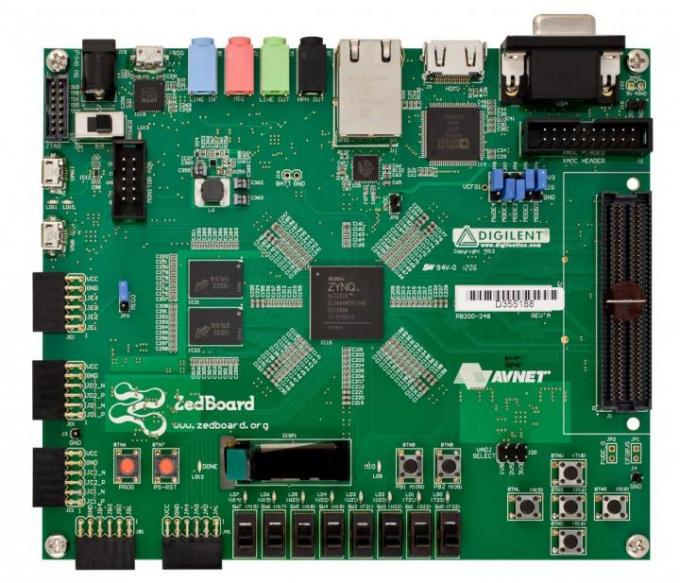
\includegraphics[width=8cm]{figuras/zedboard}
    \caption{Zedboard visto de cima.}
\end{figure}

\subsection{Arquitetura do Zynq 7000}
Como já citado, o Zynq 7000 possui um processador \emph{dual core} Cortex A9, cada core possui sua própria MMU e memória cache L1 (instruções e dados) privada.

%layout de memoria
\subsection{OCM} O \emph{On-chip Memory} é uma pequena memória de 256KB de RAM que fica próxima ao processador, e portanto tem um acesso mais rápido. O OCM pode ser mapeado nos primeiros 256KB do espaço de endereçamento, ou nos últimos 256KB do espaço de endereçamento \cite{ug585}.


\subsection{Modos de Operação}
\label{sec:operating_modes}
A arquitetura ARMv7 conta com 9 modos de operação (7 por padrão, mais 2 com extensões habilidadas), sendo que o único modo não privilegiado é o modo de usuário, os demais modos padrão possuem o mesmo privilégio dentro do sistema\footnote{O modo hipervisor possui certas funções que os demais modos não oferecem, mas no que diz respeito à acesso a memória e execução de instruções, ainda é o mesmo privilégio}. A principal diferença entre um modo e outro é que cada modo conta com um certo subconjunto privado de registradores banqueados, visiveis somente no modo em vigência, como ilustra a imagem \ref{fig:banked}. A tabela \ref{processormode} ilustra quais são os modos de operação disponíveis \cite[p.~1139]{armarm}.
O campo ``Codificação'' é usado no registrador CPSR para se verificar ou modificar o modo de operação vigente.

\begin{table}[ht]
\centering
\begin{tabular}{ccc}
\hline\hline                        %inserts double horizontal lines
Modo do processador  & Codificação & Implementado?\\ [0.5ex] % inserts table 
%heading
\hline                  % inserts single horizontal line
User & 10000 & Sempre \\
FIQ & 10001 & Sempre \\
IRQ & 10010 & Sempre \\
Supervisor & 10011 & Sempre\\
Monitor & 10110 & Com extenções de segurança.\\
Abort & 10111 & Sempre\\
Hyp & 11010 & Com extenções de virtualização.\\
Undefined & 11011 & Sempre\\
System & 11111 & Sempre\\[1ex]
\hline %inserts single line
\end{tabular}
\caption{Modos do processador. Codificação corresponde aos bits CPSR[4:0].}
\label{tab.processormode} % is used to refer this table in the text
\end{table}

\textbf{Modo Usuário:} Modo não-privilegiado de execução. Neste modo somente é possível de se fazer acesso não privilegiado aos recursos do hardware (não prodendo acessar as áreas protegidas). Não é possível de se mudar para outro modo de operação quando neste, a não ser por eventos externos como interrupções.

\textbf{Modo Sistema:} Modo privilegiado de execução. Este modo usa os mesmos registradores que o modo usuário e nenhuma exceção leva a este modo. Somente é possível de se entrar nesse modo alterando os bits do registrador de status do sistema (CPSR); é necessário já estar em algum modo privilegiado para tal operação.

\textbf{Modo Supervisor:} É o modo padrão para no qual processador entra quando uma exceção do tipo \emph{Supervisor Call} é recebida.
Para gerar um \emph{Supervisor Call}, usa-se a instrução \verb+svc+. O processador entra neste modo ao se resetar.

\textbf{Modo Abort:} Modo que o processador entra quando recebe uma interrupção do tipo \emph{prefetch abort} ou \emph{data abort}.

\textbf{Modo Indefinido:} Modo que o processador entra quando se tenta executar uma instrução não definida.

\textbf{Modo FIQ:} Modo que o processador entra quando recebe uma interrupção FIQ.

\textbf{Modo IRQ:} Modo que o processador entra quando recebe uma interrupção IRQ.

\textbf{Modo Hipervisor:} Este modo possui alguns privilégios a mais que os demais modos, mas somente existe quando as extenções de virtualização estão ativas (fora do escopo deste trabalho).

\textbf{Modo Monitor:} Modo que o processador entra quando recebe uma interrupção \emph{Secure Monitor Call}, \verb+SMC+. Este modo está fora do escopo do trabalho.


\begin{figure}[ht!]
	\centerline{
    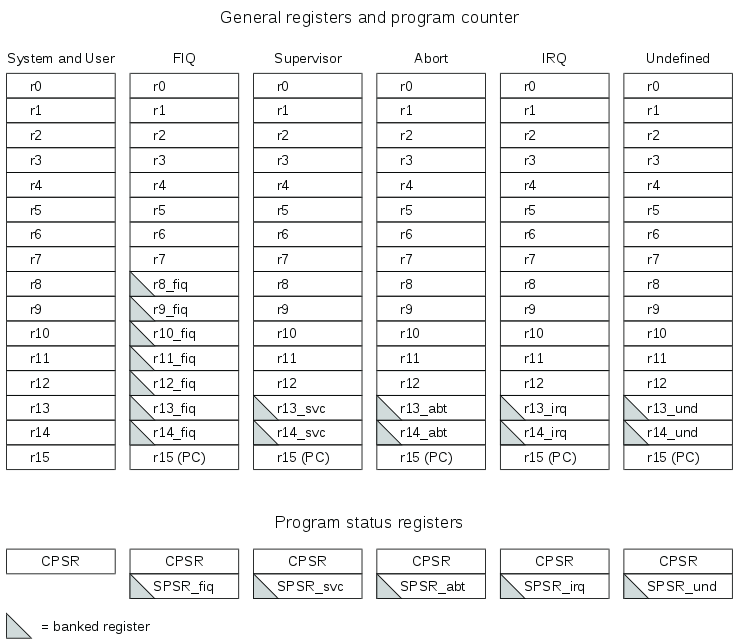
\includegraphics[width=12cm]{figuras/banked_registers}
	}
    \caption{Registradores banqueados.}
	\label{fig:banked}
\end{figure}



\subsection{GIC}
O GIC (\emph{Generic Interrupt Controller}) é um componente que centraliza e administra todas as interrupções do sistema, ativando, desativando, mascarando e priorizando as fontes de interrupção.


\subsection{Tipos de Interrupção} %ug585 p. 192
\label{sec:interrupt}
\textbf{Interrupção Gerada por Software: }
Cada CPU pode se interromper, interromper outra CPU, ou ambas CPUs usando SGIs (\emph{Software Generated Interrupts}). Existem 16 interrupções geradas por software, que podem ser geradas escrevendo o número da interrupção ([0-15]), junto com o número da CPU alvo no registrador ICDSGIR. Esta escrita ocorre dentro do barramento privado da própria CPU. Cada CPU possui seu próprio conjunto privado de registradores de SGIs para gerarem uma (ou mais) das 16 SGIs possíveis \cite[p.~216]{ug585.1.7}. É possível limpar uma interrupção lendo o registrador ICCIAR (\emph{Interrupt Acknowledge}) ou escrevendo 1 nos bits correspondentes do registrador ICDICPR (\emph{Interrupt Clear-Pending}).
\\\\
\textbf{Interrupções de Periféricos Privados da CPU: }
Cada CPU está conectada a um conjunto privado de 5 interrupções de periféricos, são eles: Relógio Global (\emph{Global Timer}), nFIQ (\emph{Fast Interrupt}), Relógio privado da CPU, \emph{Watchdog} privado da CPU e nIRQ (interrupção vinda da lógica programável).
\\\\
\textbf{Interrupções de Periféricos Compartilhados: }
Existem cerca de 60 interrupções de diversos modulos que podem ser roteadas para um ou ambos processadores, ou para a lógica programável. O GIC é responsável por administrar estas interrupções.


Há também as interrupções\footnote{Na nomenclatura do manual, usa-se o termo exceção para os 6 diferentes tipos de interrupção, e de interrupção os diferentes tipos de interrupção IRQ ou FIQ (as categorias de interrupção descritas acima são do tipo IRQ). Durante este trabalho preferiu-se usar apenas o nome interrupção, pois assim não há ambiguidade com a palavra exceção no contexto de linguagens de programação.} geradas por alguma exceção, i.e. algum evento inesperado no fluxo de execução. Além das interrupções IRQ (contempladas acima) existem mais 5 tipos interrupções que devem ser contempladas. São elas:

\textbf{FIQ \emph{Fast Interrupt}:} O modo FIQ possui um número maior de registradores banqueados que os demais modos (R8 até R13, além do SP, LR e SPSR), fazendo com que não seja necessário fazer troca de contexto. FIQs também tem mais alta prioridade que qualquer IRQ, pontanto este tipo de interrupção é apropriado para aplicações de tempo real de usuário único. Se multiplas aplicações tempo real usarem FIQ, pode haver conflitos de interesse que podem fazer um processo perder um \emph{deadline} \cite[p.~66]{armarm}.

%FIQ mode is designed for efficient use by a single owner, using R8_fiq - R13_fiq as global variables. 
%In addition, unlike IRQs, FIQs are not disabled by other exceptions (apart from reset), making them 
%the preferred type for real time interrupts, when other exceptions are being used routinely, such as 
%virtual memory or instruction emulation. IRQs may be disabled for unacceptably long periods of time 
%while these needs are being serviced.
%However, if more than one real-time interrupt source is required, there is a conflict of interest. The 
%new mechanism allows multiple FIQ sources and minimizes the period with FIQs disabled, greatly 
%reducing the interrupt latency penalty. The FIQ mode registers can be allocated to the highest priority 
%FIQ as a single owner
%ARM ARM p. 66.

\textbf{Instrução não definida (\emph{Undefined Instruction}):} 
Há duas situações que geram esta interrupção: Quando se executa instruções de coprocessador que não são reconhecidas por este, ou quando se executa instruções que não possuem significado para o processador \cite[p.~36]{armarm}. Normalmente este tipo de interrupção acontecerá quando o processador estiver lendo e tentando executar lixo de memória.


\textbf{\emph{Prefetch Abort: }} Interrupção que leva ao modo \emph{Abort}. Este tipo de interrupção é sinalizado pelo sistema de memória (MMU). Através da MMU, é possível de se marcar certas regiões de memória como não executáveis; isto é importante de se fazer em regiões de memória que possuem dados sensíveis, de modo que quando o processador tentar ler aquela área para executar num futuro próximo, a MMU envia um sinal invalidando aquilo que foi lido. Quando o processador tenta executar uma instrução que tenha sido anteriormente invalidada, uma interrupção do tipo \emph{prefetch} ocorre \cite[p.~58]{armarm}. Note que é possível do processador ler aquela região para executar em seguida, mas ainda não gerar esta interrupção; isto ocorre quando o fluxo é desviado antes da tentativa de executar aquela instrução (por um \emph{branch} por exemplo).

\textbf{\emph{Data Abort:}} Assim como a \emph{prefetch abort}, esta interrupção também leva ao modo \emph{Abort} (e somente estas duas interrupções). Este tipo de interrupção pode acontecer quando uma instrução tenta acessar uma região de memória que o modo atual de execução não tenha permissão para acessar. Acesso a regiões de memória virtual não mapeadas pela MMU também geram esta interrupção.


%Source: http://infocenter.arm.com/help/index.jsp?topic=/com.arm.doc.dui0068b/BABFCEEG.html
\textbf{Interrupção de Software: } Existe uma instrução no assembly do ARMv9 que permite que seja feita uma interrupção de software (\verb+swi+). Esta instrução pode ser acompanhada de um número de 8 bits, significando que é possível se criar 256 interrupções de software diferentes. Esta interrupção leva ao modo supervisor.

\subsection{(\emph{Timers})}
Cada um dos \emph{cores} possui um \emph{timer} privado de 32 bits e ambos \emph{cores} compartilham um \emph{timer} global de 64 bits. Estes \emph{timers} trabalham numa frequência sempre igual à metade da frequência da CPU.
No nível de sistema (\emph{sistem-level (PS)}), há dois \emph{timers} triplos, cujas frequências são sempre um quarto ou um sexo da frequência da CPU.




\subsection{\emph{Clocks}}

%30 <= PS_CLK <= 60MHZ
O \emph{clock} principal do sistema, chamado aqui de PS\_CLK (\emph{Processing System Clock}), é responsável por alimentar as 3 PLLs\footnote{\emph{Phase-Locked Loop}. É um sistema de controle que gera uma saída cuja fase é relacionada à fase do sinal de entrada. Pode ser usada para estabilizar um sinal e também multiplica-lo.} do sistema, sendo cada uma dessas PLLs responsável por uma parte diferente do sistema \cite[p.~622]{ug585}. O PS\_CLK é um \emph{clock} de baixa frequência, ficando entre 30 a 60 MHz (PS\_CLK é igual a 33.33 MHz no caso da Zedboard), sendo este multiplicado por cada uma das 3 PLLs para que o sistema funcione com velocidades maiores\footnote{Este clock pode ser multiplicado por um número de 1 a 127, e é multiplicado por 26 por padrão.}. As 3 PLLs são:

\begin{itemize}
	\item \textbf{I/O PLL:} Responsável por produzir o sinal de \emph{clock} para os dispositivos de entrada e saída.
	\item \textbf{DDR PLL:} Responsável por produzir o sinal de \emph{clock} para as memórias da plataforma.
	\item \textbf{ARM PLL:} Responsável por produzir o sinal de \emph{clock} do restante do sistema, incluindo os processadores.
\end{itemize}

A FPGA da Zedboard possui um \emph{clock} próprio e exclusivo. A figura \ref{fig:clocks} ilustra como estão dispostos estes \emph{clocks}.

\begin{figure}[ht!]
	\centerline{
    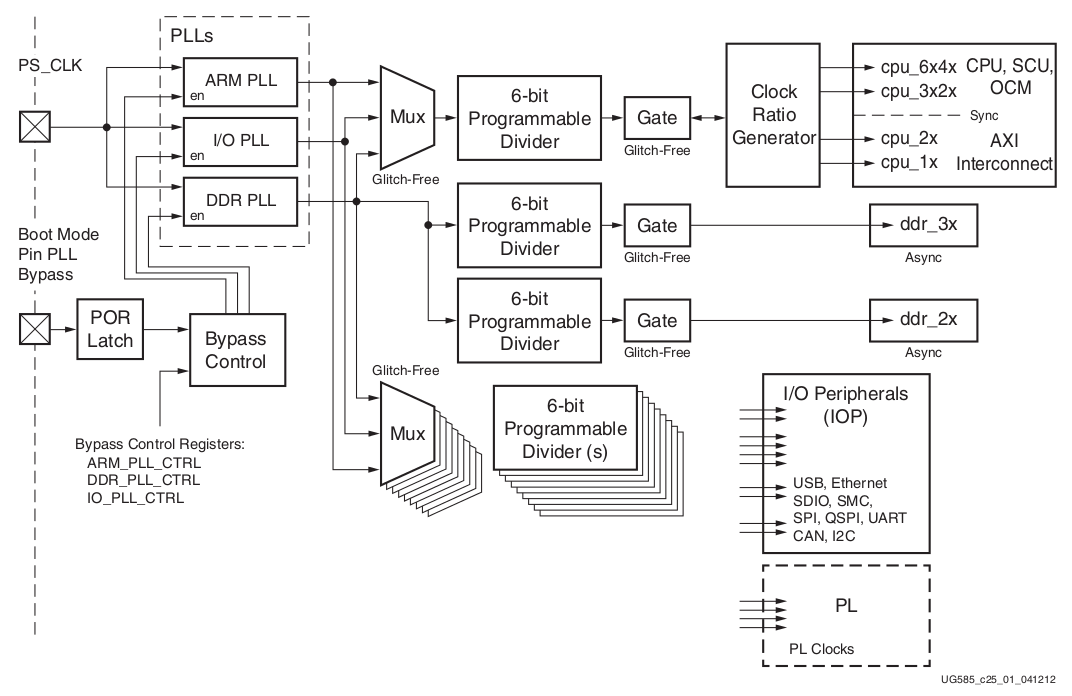
\includegraphics[width=13cm]{figuras/clocks}
	}
    \caption{Diagrama de blocos dos \emph{clocks} disponíveis no Zynq. Note os \emph{clocks} da tabela \ref{tab:clocks} no canto superior direito da imagem.}
	\label{fig:clocks}
\end{figure}

A Zedboard pode operar em dois modos (ou velocidades), denominados pela pela razão 6:3:2:1 e 4:2:2:1, abreviados como 6:2:1 e 4:2:1. Para alternar entre estes dois modos de velocidade, basta escrever 1 ou 0 no registrador CLK\_621\_TRUE. Estes números indicam quantas vezes cada \emph{clock} multiplica o \emph{clock} de base CPU\_1x, sendo este CPU\_1x um \emph{clock} derivado da ARM PLL, dividido por algum fator (configurável).

Há 4 \emph{clocks} independentes, chamados de CPU\_6x4x, CPU\_3x2x, CPU\_2x e CPU\_1x. Esta nomenclatura dos \emph{clocks} indica o fator pelo qual o CPU\_1x é multiplicado em cada modo.
O primeiro número do nome indica o fator multiplicativo daquele \emph{clock} no modo 6:2:1, e o segundo número indica o fator multiplicativo no modo 4:2:1.
Por exemplo, no modo \textbf{6}:2:1, o CPU\_\textbf{6x}4x multiplica o CPU\_1x 6 vezes, e no modo \textbf{4}:2:1, o CPU\_6x\textbf{4x} multiplica o CPU\_1x 4 vezes. A tabela \ref{tab:clocks} ilustra a velocidade de cada \emph{clock} em cada um dos dois modos.

\begin{table}[ht]
	\centering
	\begin{tabular}{ccc}
		\hline\hline
		Nomenclatura & \emph{Clock Ratio Mode} & Máxima frequência da CPU\\[0.5ex]
		\hline
		CPU\_6x4x & \multirow{4}{*}{6:3:2:1} & 667 MHZ\\
		CPU\_3x2x &                          & 333 MHZ\\
		CPU\_2x   &                          & 222 MHZ\\
		CPU\_1x   &                          & 111 MHZ\\
		\hline
		CPU\_6x4x & \multirow{4}{*}{4:2:2:1} & 533 MHZ\\
		CPU\_3x2x &                          & 267 MHZ\\
		CPU\_2x   &                          & 267 MHZ\\
		CPU\_1x   &                          & 133 MHZ\\[1ex]
		\hline
	\end{tabular}
	\caption{Máximas frequências possíveis para cada configuração de \emph{clock}. Para uma lista mais completa (com as diferentes graduações de \emph{clock}), veja \cite[p.~13]{data_sheet}.}
	\label{tab:clocks}
\end{table}

%\begin{figure}[ht!]
%    \centering
%    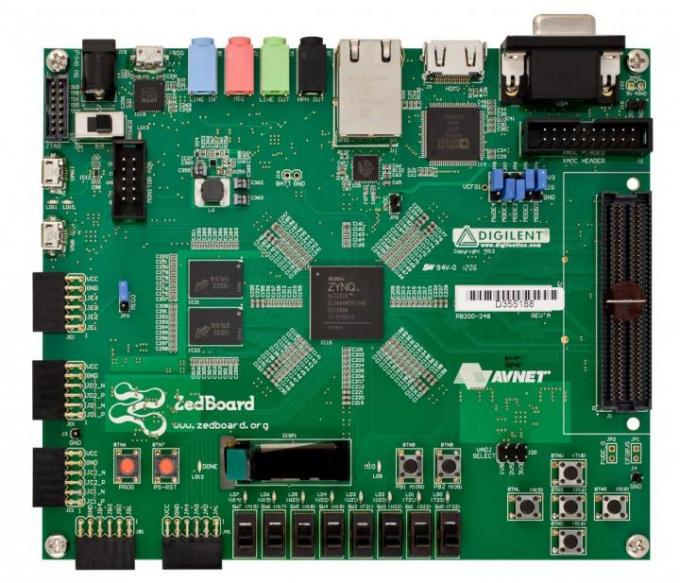
\includegraphics[width=8cm]{figuras/zedboard}
%	\caption{Arquitetura do Zynq 7000.}
%\end{figure}

\subsection{UART}
A UART (Universal Asynchronous Receiver/Transmitter) é um componente que trata da saída e entrada serial do sistema, portanto sendo o componente responsável por transmitir e receber caracteres, sendo necessário para impressão em tela, o que pode ser feito tanto por meio de um conector VGA quanto por USB (usado principalmente para depuração do código). As duas principais funções na classe da UART dentro do EPOS são justamente a put e get, para impressão e leitura de caractere, respectivamente. O Zynq possui duas UARTs.



\subsection{MMU} %http://epos.lisha.ufsc.br/EPOS+User+Guide#MMU

A MMU (\emph{Memory Managemed Unit}) é um componente responsável por gerenciar a memória de um sistema. É este componente o responsável por traduzir o endereçamento lógico em endereçamento físico. Uma das principais vantagens de seu uso é a possibilidade de proteção de memória e facilitação da escrita de aplicativos, pois estes não precisam levar em consideração o mapa de memória do SO.

%%%%%%%%
%		Get image from ug585 v1.7 p.79!
%%%%%%%%
\section{Ambiente de Desenvolvimento}

O ambiente de desenvolvimento usado para o porte foi o qemu para ARM (\verb+qemu-system-arm+), para executar o EPOS num ambiente virtualizado (emulado), pois assim pode-se usar ferramentas como o GDB para a depuração do código. O uso do GDB foi fundamental para o desenvolvimento, já que com ele era possível imprimir o valor de cada registrador em um dado ponto da execução, verificar a memória, executar instruções específicas e etc. Para compilar o EPOS foi usado \emph{cross-compilers} para ARM. As flags usadas para criar um ambiente de depuração com o qemu e o GDB foram as sequintes (com cada comando feito em um terminal diferente):
\begin{verbatim}
	qemu-system-arm -no-reboot -nographic -s -S -machine xilinx-zynq-a9\
	-cpu cortex-a9 -kernel ./img/zynq_app -fda ./img/zynq_app.img

	arm-none-eabi-gdb -ex "target remote :1234"
\end{verbatim}

O hardware real também estava disponível, e foi usado quando quando o qemu não produzia resultados confiáveis. Com o hardware real, para a depuração do código foi usado o JTAG.
